% Supplementary Material, v71 claim-calibrated language revision.
\documentclass[cmc,article,submit,moreauthors,pdftex]{Definitions/tsp}
\input{Definitions/package}
\input{Definitions/unicode}
\usepackage[OT1,OT2,T2A,T2B,T2C,T3,T5,T1]{fontenc}
\usepackage[russian,english]{babel}
\usepackage{booktabs}
\usepackage{float}
\usepackage{longtable}
\usepackage{amsmath,amssymb}
\usepackage{array}
\setlength{\headheight}{38.3pt}
\newcommand{\tabnote}[1]{\par\smallskip\noindent\begin{minipage}{\linewidth}\footnotesize\emph{Note}: #1\end{minipage}\par}
\graphicspath{{Figures/}}
\renewcommand{\thetable}{S\arabic{table}}
\renewcommand{\thefigure}{S\arabic{figure}}
\renewcommand{\thesection}{S\arabic{section}}

\continuouspages{}
\firstpage{1}
\makeatletter
\setcounter{page}{\@firstpage}
\makeatother
\pubvolume{0}
\issuenum{0}
\elocationid{0}
\articlenumber{0}
\pubyear{2026}
\copyrightyear{2026}
\datereceived{Day Month Year}
\dateaccepted{Day Month Year}
\dateonlinefirst{}
\datepublished{Day Month Year}

\Title{Supplementary Material for ``Energy-Gated DA-TPP: Batch Active Learning for Early Target Recovery in Generated Crystal Pools''}
\newcommand{\orcidauthorE}{0009-0003-3796-4444}
\Author{Yueyang Zhang\textsuperscript{1,\#}, Jinxuan Liu\textsuperscript{1,\#}, Tianyu Li\textsuperscript{2}, Xiangxiru Xiong\textsuperscript{3}, Yingjie Zhang\orcidE{}\textsuperscript{2,*} and Baohua Tan\textsuperscript{4,5,6,*}}
\AuthorNames{Yueyang Zhang, Jinxuan Liu, Tianyu Li, Xiangxiru Xiong, Yingjie Zhang and Baohua Tan}
\address{\textsuperscript{1}Hubei University of Technology, No. 28 Nanli Road, Hongshan District, Wuhan, Hubei 430068, China; \textsuperscript{2}Department of Applied Physics, The Hong Kong Polytechnic University, Hung Hom, Kowloon, Hong Kong, China; \textsuperscript{3}Department of Mathematics and Information Technology, The Education University of Hong Kong, 10 Lo Ping Road, Tai Po, New Territories, Hong Kong, China; \textsuperscript{4}School of Science (School of Chip Industry), Hubei University of Technology, Wuhan, 430068, China; \textsuperscript{5}National ``111 Research Center'' Microelectronics and Integrated Circuits, Hubei University of Technology, Wuhan, 430068, China; \textsuperscript{6}Department of Architecture and Built Environment, Faculty of Engineering, University of Nottingham, Nottingham, NG7 2RD, United Kingdom}
\corres{Corresponding Authors: Yingjie Zhang. Email: yingjieyj.zhang@connect.polyu.hk; Baohua Tan. Email: tbh@hbut.edu.cn}
\firstnote{These authors contributed equally to this work.}
\abstract{This Supplementary Material reports the parameters, source tables, and
robustness analyses supporting the main paper. Energy-Gated DA-TPP recovered seven more
surrogate targets than Greedy within the first 80 queries and retained a 14.7\%
normalized-AUTC advantage through 160 queries. An
acquisition-blind post-selection audit of 20 historical DFT attempts yielded a
nested leave-one-out ROC--AUC of 0.820 and assigned the early Gate prefix a
larger expected evaluable-target count. CHGNet
and MACE-MP completed all 640 candidates, and four generated LiCr$_2$O$_4$
candidates completed the stated PAW--PBE+$U$ relaxation--static workflow. Exact
run-identity audits, source values, arithmetic checks, crystallographic
descriptors, and a ten-seed Materials Project Mn-oxide control are retained so
that model estimates remain distinguishable from observed labels and DFT
records. Development-cohort threshold and weight sweeps, together with
same-protocol Greedy, MC-dropout, and random controls, provide the parameter and
baseline context for the main discussion. A development-selected $\gamma=0.05$
protocol was then fixed before a ten-seed held-out Gate--Greedy comparison, in
which mean AUTC through 160 queries increased from 0.2967 to 0.3223.}
\keyword{Supplementary Material; active learning; DFT evaluability; acquisition-blind evaluation; reproducibility}

\begin{document}

\section{Supplementary evidence overview}

The supplementary evidence supports a focused early-budget interpretation. In
the protocol-matched archive, Gate recovered 26 surrogate targets within 80
queries compared with 19 for Greedy. Its normalized AUTC was 12.2\% higher at an
80-query stopping horizon and 14.7\% higher through 160 queries. Both methods
ultimately recovered the same 78-target set, so the observed advantage concerns
the earlier placement of useful candidates rather than a higher endpoint
ceiling.

The downstream records provide two additional assessments of that ordering result. The
acquisition-blind evaluator assigned the 80-query Gate prefix 16.63 expected
DFT-evaluable targets, compared with 10.99 for Greedy, without influencing
selection. Separately, both MLIPs completed the full 640-candidate pool and all
four reported LiCr$_2$O$_4$ candidates completed the stated first-principles
workflow. The following sections provide the exact inputs, tables, provenance,
and scope limits for these results, including the independently initialized
held-out comparison.

\section{Target task and evidence types}

The analysis is defined by the 640-candidate Li--M--O pool, its identifiers, the
ALIGNN reference table, and the stored acquisition histories. The interval
$[-2.18,-2.02]$ eV atom$^{-1}$ contains 78 surrogate targets. It belongs to the
archived query task rather than to a stability or application criterion, and it
is fixed independently of the DFT-evaluability metric.

Retained structures and candidate identifiers establish the MatterGen-derived
provenance of the pool. Recoverable request fields are retained for provenance,
whereas acquisition analysis uses only the frozen candidate identities, ALIGNN
reference table, and stored query histories. No cross-convention conversion is
applied among generation, ALIGNN, and current DFT energies.

The source files separate three evidence types:
\begin{enumerate}
\item observed CGCNN query histories and archived DFT records;
\item an acquisition-blind machine-learning endpoint for strict DFT evaluability;
\item physical properties outside the present target-recovery and
workflow-feasibility scope.
\end{enumerate}

\begin{table}[!htbp]
\centering
\caption{Notation and evidence layers used in the frozen-pool analysis.}
\label{tab:notation}
\scriptsize
\begin{tabular}{@{}lll@{}}
\toprule
Symbol & Definition & Evidence status \\
\midrule
$\mathcal{C}$, $N$ & \pbox{0.53\textwidth}{Frozen candidate pool and its size ($N=640$)} & archived objects \\
$y_i$, $z_i$ & \pbox{0.53\textwidth}{ALIGNN reference value and interval-membership label} & reference-table oracle \\
$p_i$, $e_i$ & \pbox{0.53\textwidth}{CGCNN interval-hit probability and DFT-evaluability score} & ML estimates \\
$d_i$ & \pbox{0.53\textwidth}{Strict completion label for a historical DFT attempt} & archived DFT record \\
$\mathcal{B}_t$, $b$, $Q$ & \pbox{0.53\textwidth}{Round-$t$ batch, batch size 16, and query budget} & protocol \\
$Y_a(q)$, $H_a(q)$ & \pbox{0.53\textwidth}{Recovered targets and DFT-evaluability endpoint sum} & history; ML endpoint \\
$G_t$, $M_t$ & \pbox{0.53\textwidth}{Group concentration and standardized front margin} & gate diagnostics \\
\bottomrule
\end{tabular}
\end{table}


\section{Archived implementation and run identifiers}

The recovered parameter file and claim map are presented first so that every
later numerical statement can be traced to a frozen configuration and evidence
type.

\begin{table}[!htbp]
\centering
\caption{Recoverable settings of the archived Energy-Gated DA-TPP runs.}
\label{tab:archived-settings}
\small
\begin{tabular}{llll}
\toprule
Setting & Value & Setting & Value \\
\midrule
$M_0$ & 1.00 & $G_0$ & 0.50 \\
$\alpha$ & 0.10 & $\beta$ & 0.20 \\
$\gamma$ & 0.10 & Acquisition batch & 16 \\
MC passes & 3 & Dropout rate & 0.30 \\
Refit epochs & 10 & Learning rate & 0.001 \\
CGCNN batch size & 256 & Total query budget & 640 \\
\bottomrule
\end{tabular}
\tabnote{Values are read from the archived run configurations and remain fixed
within the stored histories. Development-cohort sensitivity and the separately
held-out protocol are reported in Tables~S12--S14.}
\end{table}


\begin{table}[!htbp]
\centering
\caption{Evidence layers and their roles in the study.}
\label{tab:claim-evidence}
\scriptsize
\begin{tabular}{@{}lll@{}}
\toprule
Evidence & Quantity assessed & Role in the study \\
\midrule
\pbox{0.23\textwidth}{Frozen query histories} & \pbox{0.34\textwidth}{Recovery of ALIGNN reference targets} & \pbox{0.27\textwidth}{Primary surrogate-ordering evidence} \\
\pbox{0.23\textwidth}{Frozen seeds 15--24 paired histories} & \pbox{0.34\textwidth}{Early AUTC and checkpoint recovery under $\gamma=0.05$} & \pbox{0.27\textwidth}{Held-out robustness assessment} \\
\pbox{0.23\textwidth}{Acquisition-blind $e_i$ scores} & \pbox{0.34\textwidth}{Estimated DFT evaluability at fixed checkpoints} & \pbox{0.27\textwidth}{Post-selection downstream assessment} \\
\pbox{0.23\textwidth}{Four completed Cr workflows} & \pbox{0.34\textwidth}{Completion, forces, geometry, moments, and energies} & \pbox{0.27\textwidth}{First-principles feasibility examples} \\
\pbox{0.23\textwidth}{Archived-prefix hash audit} & \pbox{0.34\textwidth}{Distinct archived query prefixes} & \pbox{0.27\textwidth}{Run-identity and provenance check} \\
\pbox{0.23\textwidth}{Selector-equivalence audit} & \pbox{0.34\textwidth}{Recorded route changes under the two diagnostics} & \pbox{0.27\textwidth}{Mechanism and fallback analysis} \\
\bottomrule
\end{tabular}
\end{table}


Implementation seeds 5--14 identify the formal archive. Main-text run IDs
1--10 map to them in ascending order. The original values remain in
\path{SourceData/paired_autc_at_320.csv} and the history files.

The settings in Table~S2 were loaded before each archived run and did not
change. They are reported as recovered implementation values; the separate
development-cohort sensitivity analysis is given in Table~S12.

\section{Acquisition-blind DFT-evaluability assessment}

Strict label one requires electronic and ionic convergence, a separate static
calculation, and a reproducible formation energy. Ten of the 20 archived
attempts meet all four requirements. Seven other records lack a reconstructable
energy, two contain a VASP or electronic failure, and one has an unconverged
static step.

\begin{table}[!htbp]
\centering
\caption{Nested leave-one-out assessment of the DFT-evaluability classifiers.}
\label{tab:evaluator-validation}
\scriptsize
\begin{tabular}{lrrrr}
\toprule
Model & ROC--AUC & Balanced accuracy & Brier score & Log loss \\
\midrule
Shallow gradient boosting & 0.820 & 0.700 & 0.183 & 0.545 \\
Shallow random forest & 0.660 & 0.750 & 0.234 & 0.664 \\
Regularized logistic regression & 0.540 & 0.600 & 0.258 & 0.713 \\
Laplace logistic model & 0.460 & 0.600 & 0.282 & 0.766 \\
\bottomrule
\end{tabular}
\tabnote{The development archive contains 20 DFT attempts, including 10
strictly evaluable records. Preprocessing and model selection are performed
inside each outer training fold.}
\end{table}


Shallow gradient boosting achieved the highest nested leave-one-out ROC--AUC,
0.820. Across the 20-record archive, this corresponds to correct ordering in
82\% of positive--negative record pairs used by the ROC calculation. The model
is used only as an acquisition-blind post-selection audit.

Candidate-level labels are stored in
\path{SourceData/historical_dft_binary_labels.csv}; the complete
cross-validation table is in
\path{SourceData/dft_evaluability_model_cv.csv}. The selected shallow
gradient-boosting model uses a fixed 0.50 probability threshold. Candidate IDs
and historical policy ranks are excluded from the features.

\section{Early-prefix DFT-evaluability audit}

The following table applies the frozen evaluator to the already selected Gate
and Greedy prefixes at the four reported stopping horizons.

\begin{table}[!htbp]
\centering
\caption{Surrogate target recovery and the formal DFT-evaluability endpoint at the
fixed query checkpoints.}
\label{tab:evaluability-yield}
\scriptsize
\begin{tabular}{llrrrr}
\toprule
Queries & Method & Target hits & Expected evaluable & $e_i\geq0.50$ & Mean $e_i$ \\
\midrule
80  & Gate   & 26 & 16.63 & 20 & 0.64 \\
    & Greedy & 19 & 10.99 & 12 & 0.58 \\
160 & Gate   & 54 & 33.87 & 41 & 0.63 \\
    & Greedy & 54 & 31.60 & 35 & 0.59 \\
240 & Gate   & 67 & 39.93 & 46 & 0.60 \\
    & Greedy & 69 & 40.96 & 47 & 0.59 \\
320 & Gate   & 78 & 46.51 & 53 & 0.60 \\
    & Greedy & 78 & 46.51 & 53 & 0.60 \\
\bottomrule
\end{tabular}
\tabnote{Expected evaluable is $\sum z_i e_i$ over the targets already selected
by the CGCNN policy. The acquisition-blind $e_i$ values are ML estimates and are
not supplied to Gate or Greedy.}
\end{table}


At 80 queries, Gate had recovered 26 targets with a summed expected evaluable
count of 16.63, whereas Greedy had recovered 19 targets with an expected count
of 10.99. The same early prefix also gave the larger thresholded count, 20
versus 12. The difference narrows as Greedy recovers the deferred targets and
disappears once both policies reach the common endpoint.

For a target candidate $i$, the expected contribution is $e_i$, while the
thresholded contribution is $\mathbb{I}(e_i\geq0.50)$. A non-target contributes
zero to both target-yield endpoints. Complete overlays and score provenance are
retained in
\path{SourceData/paired_dft_evaluability_detail.csv} and
\path{SourceData/dft_evaluability_scores.csv}.

\section{Query-prefix and target-set audit}

\begin{table}[H]
\centering
\caption{Identity audit of the ten archived records within each method.}
\label{tab:s-prefix-audit}
\small
\begin{tabular}{llrrr}
\toprule
Method & Queries & Stored records & Unique complete prefixes & Unique target sets \\
\midrule
Gate & 80  & 10 & 1  & 1 \\
Gate & 160 & 10 & 1  & 1 \\
Gate & 240 & 10 & 1  & 1 \\
Gate & 320 & 10 & 10 & 1 \\
Greedy & 80  & 10 & 1  & 1 \\
Greedy & 160 & 10 & 1  & 1 \\
Greedy & 240 & 10 & 1  & 1 \\
Greedy & 320 & 10 & 10 & 1 \\
\bottomrule
\end{tabular}
\tabnote{At 320 queries, complete prefixes differ only in non-target ordering.
All records within a method recover the same target set. Prefixes through 240
queries are identical within each method.}
\end{table}

The hash-level audit is retained in
\path{SourceData/target_set_identity_audit.csv} and
\path{SourceData/target_set_identity_summary.csv}. Because each method has one
distinct complete prefix through 240 queries, the stored IDs do not provide
replicates for an inferential paired test.

\section{Reconstructed early-horizon AUTC advantage}

\begin{table}[H]
\centering
\caption{Normalized AUTC for the canonical recoverable Gate and Greedy trajectories.}
\label{tab:s-autc-horizons}
\small
\begin{tabular}{@{}rrrr@{}}
\toprule
Stopping budget & Gate AUTC & Greedy AUTC & Relative Gate difference \\
\midrule
80  & 0.1410 & 0.1256 & $+12.2\%$ \\
160 & 0.3205 & 0.2795 & $+14.7\%$ \\
240 & 0.4692 & 0.4504 & $+4.2\%$ \\
320 & 0.5827 & 0.5718 & $+1.9\%$ \\
\bottomrule
\end{tabular}

\tabnote{AUTC uses the left-continuous 16-query-batch sum and the 78-target
ceiling. The relative difference is $(\mathrm{Gate}/\mathrm{Greedy}-1)\times
100\%$.}
\end{table}

Gate exceeded Greedy in normalized AUTC at every reported stopping horizon. The
relative differences were 12.2\%, 14.7\%, 4.2\%, and 1.9\% through 80, 160,
240, and 320 queries, respectively. The largest advantage therefore occurs in
the early-budget regime targeted by the method.

Candidate-level histories were recomputed with a left-continuous 16-query-batch
sum at stopping budgets of 80, 160, 240, and 320. Input trajectories and values
are retained in
\path{SourceData/paired_cgcnn_histories.csv} and
\path{SourceData/v50_autc_checkpoints.csv}. The 20 stored 320-query row values
and implementation seed mapping remain in
\path{SourceData/paired_autc_at_320.csv}. Differences after the identical early
prefixes do not create independent replicates.

\section{Complete full-pool MLIP execution}

Both low-fidelity models were executed for every candidate. Figure~\ref{fig:s-mlip-runtime}
shows the resulting per-candidate wall-time distributions in the recorded
environment.

\begin{figure}[H]
\centering
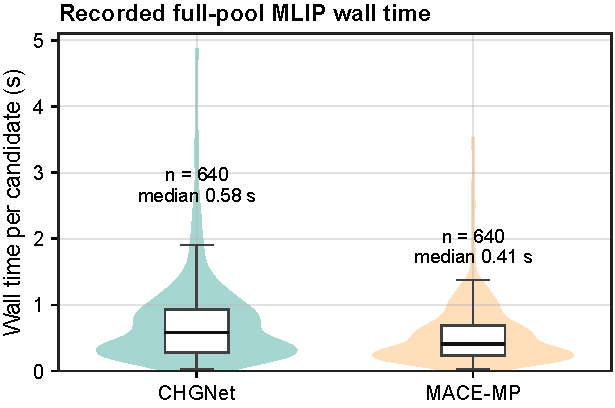
\includegraphics[width=0.64\textwidth]{FigureS_v50_mlip_runtime.pdf}
\caption{Per-candidate wall times for 640 CHGNet and 640 MACE-MP evaluations.
Boxes show the interquartile range and median within each violin. Values come
from the archived MLIP environment and are not normalized to DFT hardware.}
\label{fig:s-mlip-runtime}
\end{figure}

The two models produced 1,280 complete records in 781.545 s of aggregate wall
time. Median per-candidate values were 0.582 s for CHGNet and 0.408 s for
MACE-MP.
Candidate-level values are supplied in
\path{SourceData/mlip_full_pool_results.csv}, whose SHA-256 is
\texttt{37fc2a9ce0f7eb9c4d914b5f347f0c127a32754edb1bc38c06748f7fb7a51892}.

For the ten records with reconstructable DFT energies, leave-one-out offset
correction of MACE-MP produced an MAE of 0.0145 eV atom$^{-1}$ and an RMSE of
0.0159 eV atom$^{-1}$. Seven observed DFT values fell inside the nominal 95\%
intervals. Candidate-level outer-fold predictions are retained in
\path{SourceData/energy_calibration_best_oof.csv}.

\section{Descriptive six-policy archive}

The legacy archive preserves one complete trajectory for each of the six
implemented policies. Its checkpoint counts and evaluator overlay are reported
below as descriptive evidence.

\begin{table}[H]
\centering
\caption{Descriptive DFT-evaluability endpoint on the single archived
six-policy histories.}
\label{tab:legacy-baselines}
\scriptsize
\begin{tabular}{lrrrrrrrr}
\toprule
& \multicolumn{2}{c}{80 queries} & \multicolumn{2}{c}{160 queries}
& \multicolumn{2}{c}{240 queries} & \multicolumn{2}{c}{320 queries} \\
\cmidrule(lr){2-3}\cmidrule(lr){4-5}\cmidrule(lr){6-7}\cmidrule(lr){8-9}
Method & Target & Exp. eval. & Target & Exp. eval. & Target & Exp. eval. & Target & Exp. eval. \\
\midrule
Energy-Gated DA-TPP & 33 & 20.20 & 50 & 29.78 & 69 & 40.66 & 78 & 46.51 \\
Explore & 29 & 17.32 & 44 & 26.05 & 60 & 35.44 & 74 & 43.60 \\
Predicted-Target Greedy & 27 & 16.36 & 47 & 28.78 & 69 & 40.96 & 78 & 46.51 \\
MC Dropout & 8 & 4.44 & 27 & 14.42 & 36 & 20.43 & 49 & 28.56 \\
Modulus/Gradient-Norm & 10 & 5.54 & 20 & 9.22 & 39 & 18.83 & 58 & 32.40 \\
Random Sampling & 6 & 4.29 & 18 & 11.30 & 26 & 15.57 & 39 & 22.73 \\
\bottomrule
\end{tabular}
\tabnote{Each row is one historical trajectory and is provided only as
descriptive context. Exp. eval. is the expected number of target candidates
scored as DFT-evaluable by the acquisition-blind endpoint. These histories are not paired
replicates of the formal Gate--Greedy archive.}
\end{table}


Gate and Greedy in Table~\ref{tab:legacy-baselines} are historical single-run
records, distinct from the matched archive used for the primary comparison.
They preserve the older comparison with Explore, MC Dropout,
Modulus/Gradient-Norm, and Random Sampling. The table is descriptive.

\section{First-principles protocol for four completed candidates}

The first-principles set contains C079-1, C126-0, C196-1, and C234-3. These four
records are separate from the 20 attempts used by the DFT-evaluability model and
were not sampled as a Gate--Greedy yield comparison.

All four calculations used VASP 6.5.1, current PAW-PBE datasets, Dudarev
PBE+$U$ with $U_{\mathrm{eff}}(\mathrm{Cr})=3.7$ eV, and
\texttt{ENCUT}$=649$ eV. Relaxations used \texttt{EDIFF}$=10^{-6}$ eV,
\texttt{EDIFFG}$=-0.05$ eV \AA$^{-1}$, \texttt{IBRION}$=2$,
\texttt{ISIF}$=3$, \texttt{NSW}$=200$, \texttt{ISPIN}$=2$,
\texttt{ISMEAR}$=0$, \texttt{SIGMA}$=0.05$ eV,
\texttt{LASPH}=TRUE, and \texttt{LMAXMIX}$=4$. Independent statics used the
relaxed structure with \texttt{IBRION}$=-1$ and \texttt{NSW}$=0$.
Gamma-centred meshes were generated with an approximately
0.15~\AA$^{-1}$ reciprocal-spacing rule: $15\times11\times7$ for C079-1,
$15\times10\times9$ for C126-0, and $16\times16\times5$ for C196-1 and
C234-3.

POTCAR text is not redistributed. The archived SHA-256 identifiers are
\texttt{201875120238865c...fbb95b} for Li,
\texttt{836672959fc86f3b...9bd744b} for Cr, and
\texttt{8a74b9a1f5fdb3d...a3eea64} for O; the complete values are retained in
\path{SourceData/DFT_completed_candidates_report_zh.md}.

\section{Completed first-principles workflows and energy reconstruction}

All four LiCr$_2$O$_4$ candidates completed full cell-and-ion relaxation and a
separate static calculation. Their reconstructed formation energies span
$-2.1676$ to $-2.0336$ eV atom$^{-1}$, maximum residual forces remain below the
0.05 eV \AA$^{-1}$ stopping criterion, and no automated cell-collapse flag was
raised.

\begin{table}[H]
\centering
\caption{Completed LiCr$_2$O$_4$ first-principles feasibility calculations.}
\label{tab:s-dft-candidates}
\tablesize{\scriptsize}
\resizebox{\textwidth}{!}{\begin{tabular}{@{}lrrrrrr@{}}
\toprule
Candidate & $E_f$ (eV atom$^{-1}$) & $F_{\max}$ (eV \AA$^{-1}$) &
$\Delta V$ (\%) & Shortest distance (\AA) &
Moment ($\mu_{\mathrm{B}}$ cell$^{-1}$) & Gap (eV) \\
\midrule
C079-1 & $-2.164905884$ & 0.045128 & $+2.918$ & 1.917646 & 4.937 & 0.0035 \\
C126-0 & $-2.167618531$ & 0.034407 & $-1.358$ & 1.938847 & 4.922 & 0.0010 \\
C196-1 & $-2.033635033$ & 0.033610 & $+0.962$ & 1.724317 & 4.864 & 0.0004 \\
C234-3 & $-2.033665270$ & 0.044104 & $+0.586$ & 1.724466 & 4.864 & 0.0015 \\
\bottomrule
\end{tabular}
}
\tabnote{The reported gap is a near-zero-gap diagnostic. The magnetic moment
belongs to the tested initialization and is not a magnetic-ground-state
assignment.}
\end{table}

The internally consistent formation energy is
\begin{equation}
E_f =
\frac{E_{\mathrm{LiCr_2O_4}}-\mu_{\mathrm{Li}}
-2\mu_{\mathrm{Cr}}-2E_{\mathrm{O_2}}}{7}.
\end{equation}
The retained reference energies are
$\mu_{\mathrm{Li}}=-1.90574968$ eV atom$^{-1}$,
$\mu_{\mathrm{Cr}}=-6.16417684$ eV atom$^{-1}$, and
$E_{\mathrm{O_2}}=-9.89314292$ eV molecule$^{-1}$. Two independent
recalculation scripts agree within $10^{-15}$ eV atom$^{-1}$. The check
establishes arithmetic consistency inside this protocol. Because no validated
compatibility mapping to Materials Project or ALIGNN energies is available, no
cross-scale conversion is applied
(archived status: \texttt{same\_scale\_status=UNRESOLVED}).

All four relaxations satisfy $F_{\max}\leq0.05$ eV \AA$^{-1}$ without an
automated cell-collapse flag, and all four final static calculations completed
from converged relaxed structures. Restart provenance and the recorded C234-3
lattice warning are retained in the source archive. The calculations assess
workflow completion and local relaxation under the stated protocol; phase
stability requires a separate competing-phase analysis.

Final structures were parsed from the retained static \texttt{vasprun.xml}
records and exported as \path{Structures/C079-1_final.cif},
\path{Structures/C126-0_final.cif}, \path{Structures/C196-1_final.cif}, and
\path{Structures/C234-3_final.cif}. The source XML path, XML hash, CIF hash,
lattice parameters, site count, and final volume are listed in
\path{SourceData/v50_final_structure_provenance.csv}.

\section{Crystallographic descriptors and structure matching}

The final CIFs were re-read independently and analysed at symmetry tolerances
of 0.01, 0.05, and 0.10~\AA. Table~\ref{tab:s-crystallography} gives the two
endpoint assignments together with the cell dimensions. This tolerance report
prevents a single symmetry setting from being treated as an exact physical
classification.

\begin{table}[H]
\centering
\caption{Lattice and symmetry descriptors of the four relaxed LiCr$_2$O$_4$
candidates.}
\label{tab:s-crystallography}
\tablesize{\scriptsize}
\resizebox{\textwidth}{!}{\begin{tabular}{lrrrrll}
\toprule
Candidate & $a$ (\AA) & $b$ (\AA) & $c$ (\AA) & $V$ (\AA$^3$) & SG (0.01 \AA) & SG (0.10 \AA) \\
\midrule
C079-1 & 2.946 & 3.824 & 6.706 & 75.547 & Pm & Pmm2 \\
C126-0 & 2.939 & 5.073 & 5.740 & 73.810 & Cm & C2/m \\
C196-1 & 3.199 & 3.199 & 8.644 & 74.807 & R3m & R3m \\
C234-3 & 3.201 & 3.201 & 8.409 & 74.642 & P3m1 & P3m1 \\
\bottomrule
\end{tabular}
}
\tabnote{Space groups were assigned from the final CIFs with pymatgen at the
stated symmetry tolerance. Complete lattice angles and the intermediate
0.05~\AA\ result are retained in
\path{SourceData/v60_crystallographic_descriptors.csv}.}
\end{table}

Pairwise comparisons used StructureMatcher with
$l_{\mathrm{tol}}=0.2$, $s_{\mathrm{tol}}=0.3$, an angle tolerance of
$5^{\circ}$, primitive-cell reduction, and scale normalization. No pair matched
under this recorded configuration. The six pairwise decisions are retained in
\path{SourceData/v60_structure_matcher_pairs.csv}; this result supports
structural distinctness under the stated matcher and is not a proof of different
thermodynamic phases.

\section{Materials Project Mn-oxide control}

The control uses a 640-candidate Mn-bearing oxide pool and Materials Project
formation-energy labels. The frozen interval $[-2.59,-2.47]$ eV atom$^{-1}$
contains 111 targets. Corrected seeds 5--14 use prediction-loader
\texttt{shuffle=False}, explicit candidate-ID reindexing, batch size 16, and a
320-query budget. The element-system map contains 614 groups, including 588
singletons, and has a maximum group size of two.

Table~\ref{tab:s-mnoxide-control} reports every corrected seed before the
aggregate result is discussed. Gate and Greedy have identical batch membership
and checkpoint recovery in every seed.

\begin{table}[H]
\centering
\caption{Per-seed Materials Project Mn-oxide control for Gate and Greedy.}
\label{tab:s-mnoxide-control}
\tablesize{\scriptsize}
\resizebox{\textwidth}{!}{\begin{tabular}{rrrrrrrr}
\toprule
Seed & AUTC (both) & $R_{80}$ & $R_{160}$ & $R_{240}$ & $R_{320}$ & Direct & Correction \\
\midrule
5 & 0.450000 & 26 & 50 & 81 & 103 & 19 & 1 \\
6 & 0.450901 & 26 & 50 & 81 & 103 & 20 & 0 \\
7 & 0.454505 & 26 & 50 & 81 & 106 & 20 & 0 \\
8 & 0.450450 & 26 & 50 & 81 & 102 & 20 & 0 \\
9 & 0.450901 & 26 & 50 & 81 & 101 & 20 & 0 \\
10 & 0.450450 & 26 & 50 & 81 & 102 & 20 & 0 \\
11 & 0.450000 & 26 & 50 & 81 & 99 & 20 & 0 \\
12 & 0.450000 & 26 & 50 & 81 & 100 & 20 & 0 \\
13 & 0.451351 & 26 & 50 & 81 & 100 & 20 & 0 \\
14 & 0.450000 & 26 & 50 & 81 & 101 & 20 & 0 \\
\bottomrule
\end{tabular}
}
\tabnote{AUTC and recovery values are identical for Gate and Greedy within each
seed. ``Direct'' and ``Correction'' refer to Gate's 20 batch decisions. The
single correction in seed 5 reordered candidates within the same batch but
caused no effective replacement.}
\end{table}

The ten-seed aggregate normalized AUTC was
$0.450856\pm0.001367$ for both policies. Gate retained the direct route in
199/200 batches, and no correction changed batch membership. Source-backed
metrics, trajectories, pairing decisions, the full group map, and its inventory
are retained in \path{SourceData/mnoxide_corrected_seed_metrics.csv},
\path{SourceData/mnoxide_recovery_trajectories.csv},
\path{SourceData/mnoxide_seed_pairing_audit.csv},
\path{SourceData/mnoxide_element_system_groups.csv}, and
\path{SourceData/mnoxide_group_inventory.csv}.

\section{Development-cohort gate sensitivity}

The development-cohort analysis varied the two routing thresholds on a
$3\times3$ grid and varied each diversity weight one factor at a time around
the archived setting. All configurations used the same 640-candidate pool,
batch size 16, 30 MC-dropout passes, and seeds 0--4. The archived result was not
retroactively changed. The best tested development value for the group-reuse
penalty, $\gamma=0.05$, was instead frozen for a separate held-out comparison;
all other settings were retained. Table~\ref{tab:s-parameter-sensitivity}
reports every tested configuration before the aggregate interpretation in the
main text.

\begin{table}[H]
\centering
\caption{Complete development-cohort gate-parameter sensitivity.}
\label{tab:s-parameter-sensitivity}
\tablesize{\scriptsize}
\resizebox{\textwidth}{!}{\begin{tabular}{llccccc}
\toprule
Sweep & Setting & AUTC$_{160}$ & AUTC$_{640}$ & $R_{80}$ & Correction rounds & Unique paths \\
\midrule
Threshold & $M_0=0.75,\ G_0=0.40$ & $0.3038 \pm 0.0144$ & $0.7928 \pm 0.0092$ & $26.2 \pm 2.8$ & $39.2 \pm 0.8$ & 5/5 \\
Threshold & $M_0=0.75,\ G_0=0.50$ & $0.3090 \pm 0.0074$ & $0.7913 \pm 0.0091$ & $27.0 \pm 2.2$ & $34.6 \pm 1.3$ & 5/5 \\
Threshold & $M_0=0.75,\ G_0=0.60$ & $0.3038 \pm 0.0117$ & $0.7899 \pm 0.0056$ & $26.2 \pm 2.3$ & $31.0 \pm 2.0$ & 5/5 \\
Threshold & $M_0=1.00,\ G_0=0.40$ & $0.3038 \pm 0.0144$ & $0.7928 \pm 0.0092$ & $26.2 \pm 2.8$ & $39.4 \pm 0.9$ & 5/5 \\
Threshold & $M_0=1.00,\ G_0=0.50$ & $0.3090 \pm 0.0074$ & $0.7913 \pm 0.0091$ & $27.0 \pm 2.2$ & $34.8 \pm 1.1$ & 5/5 \\
Threshold & $M_0=1.00,\ G_0=0.60$ & $0.3038 \pm 0.0117$ & $0.7899 \pm 0.0056$ & $26.2 \pm 2.3$ & $31.4 \pm 1.3$ & 5/5 \\
Threshold & $M_0=1.25,\ G_0=0.40$ & $0.3038 \pm 0.0144$ & $0.7928 \pm 0.0092$ & $26.2 \pm 2.8$ & $39.4 \pm 0.9$ & 5/5 \\
Threshold & $M_0=1.25,\ G_0=0.50$ & $0.3090 \pm 0.0074$ & $0.7913 \pm 0.0091$ & $27.0 \pm 2.2$ & $35.2 \pm 1.1$ & 5/5 \\
Threshold & $M_0=1.25,\ G_0=0.60$ & $0.3038 \pm 0.0117$ & $0.7899 \pm 0.0056$ & $26.2 \pm 2.3$ & $32.4 \pm 1.5$ & 5/5 \\
Weight & $\alpha=0.05,\ \beta=0.20,\ \gamma=0.10$ & $0.3008 \pm 0.0205$ & $0.7902 \pm 0.0099$ & $25.6 \pm 2.8$ & $36.2 \pm 1.3$ & 5/5 \\
Weight & $\alpha=0.20,\ \beta=0.20,\ \gamma=0.10$ & $0.1977 \pm 0.0463$ & $0.7225 \pm 0.0216$ & $16.2 \pm 4.8$ & $35.6 \pm 2.5$ & 5/5 \\
Weight & $\alpha=0.10,\ \beta=0.20,\ \gamma=0.10$ & $0.3090 \pm 0.0074$ & $0.7913 \pm 0.0091$ & $27.0 \pm 2.2$ & $34.8 \pm 1.1$ & 5/5 \\
Weight & $\alpha=0.10,\ \beta=0.10,\ \gamma=0.10$ & $0.3069 \pm 0.0056$ & $0.7919 \pm 0.0060$ & $27.6 \pm 1.5$ & $35.2 \pm 1.5$ & 5/5 \\
Weight & $\alpha=0.10,\ \beta=0.40,\ \gamma=0.10$ & $0.3151 \pm 0.0300$ & $0.7909 \pm 0.0149$ & $27.2 \pm 2.9$ & $35.4 \pm 1.5$ & 5/5 \\
Weight & $\alpha=0.10,\ \beta=0.20,\ \gamma=0.05$ & $0.3292 \pm 0.0087$ & $0.7985 \pm 0.0047$ & $30.0 \pm 1.2$ & $34.8 \pm 1.5$ & 5/5 \\
Weight & $\alpha=0.10,\ \beta=0.20,\ \gamma=0.20$ & $0.2900 \pm 0.0121$ & $0.7822 \pm 0.0078$ & $25.0 \pm 1.7$ & $35.6 \pm 1.5$ & 5/5 \\
\bottomrule
\end{tabular}
}
\tabnote{Values are mean $\pm$ sample SD across seeds 0--4. AUTC$_{160}$
uses the trajectory truncated at 160 queries; AUTC$_{640}$ uses the complete
finite-pool trajectory. ``Unique paths'' gives the number of distinct complete
candidate-sequence hashes among the five seeds.}
\end{table}

Per-seed metrics, aggregate values, query-sequence hashes, the repeated-center
reproducibility check, and output hashes are retained in
\path{SourceData/v60_parameter_sensitivity_per_seed.csv},
\path{SourceData/v60_parameter_sensitivity_summary.csv},
\path{SourceData/v60_parameter_sensitivity_seed_audit.csv},
\path{SourceData/v60_parameter_sensitivity_reproducibility_audit.csv}, and
\path{SourceData/v60_parameter_sensitivity_output_sha256.csv}.

\section{Same-protocol low-cost baselines}

To separate the gate comparison from the historical single-run archive, three
low-cost selectors were rerun on the same development cohort used for the
sensitivity analysis. Energy-Gated DA-TPP, Predicted-Target Greedy, MC Dropout,
and Random Sampling received the same checkpoint, matched seed policy, model
schedule, batch size, query budget, and 30-pass predictive output. Their
source-backed results are introduced in Table~\ref{tab:s-same-protocol-baselines}.

\begin{table}[H]
\centering
\caption{Same-protocol development-cohort comparison with low-cost baselines.}
\label{tab:s-same-protocol-baselines}
\tablesize{\scriptsize}
\resizebox{\textwidth}{!}{\input{Tables/generated/table_v67_same_protocol_baselines}}
\tabnote{Values are mean $\pm$ sample SD across seeds 0--4. The Gate row uses
the archived $\gamma=0.10$ setting; the development-selected $\gamma=0.05$
protocol is evaluated on held-out seeds in Table~S14.}
\end{table}

Candidate-level outputs and audit hashes are retained in
\path{SourceData/v60_same_protocol_baselines_per_seed.csv},
\path{SourceData/v60_same_protocol_baselines_summary.csv},
\path{SourceData/v60_same_protocol_baselines_seed_audit.csv}, and
\path{SourceData/v60_same_protocol_gate_greedy_paired.csv}, together with
\path{SourceData/v60_same_protocol_baselines_output_sha256.csv}.

\section{Frozen held-out Gate--Greedy evaluation}

After the development sweep was complete, $\gamma=0.05$ and all remaining
protocol fields were frozen before seeds 15--24 were evaluated. Each seed used a
different initial labelled set; both methods shared that set and the same
seed-specific training and inference schedule. All 20 runs completed 640-query
trajectories, and each method produced ten distinct complete sequence hashes.
Table~\ref{tab:s-gamma005-holdout} reports the paired early-budget values.

\begin{table}[H]
\centering
\caption{Per-seed frozen held-out comparison for Energy-Gated DA-TPP and
Predicted-Target Greedy.}
\label{tab:s-gamma005-holdout}
\tablesize{\scriptsize}
\resizebox{\textwidth}{!}{\begin{tabular}{rrrrrrrr}
\toprule
Seed & Gate AUTC$_{160}$ & Greedy AUTC$_{160}$ & $\Delta$AUTC$_{160}$ & Gate $R_{80}$ & Greedy $R_{80}$ & Gate $R_{160}$ & Greedy $R_{160}$ \\
\midrule
15 & 0.3462 & 0.3385 & +0.0077 & 31 & 26 & 54 & 52 \\
16 & 0.3269 & 0.2897 & +0.0372 & 26 & 24 & 54 & 53 \\
17 & 0.3667 & 0.3179 & +0.0487 & 33 & 27 & 57 & 49 \\
18 & 0.3103 & 0.2436 & +0.0667 & 27 & 21 & 54 & 43 \\
19 & 0.2769 & 0.2808 & $-0.0038$ & 25 & 25 & 48 & 47 \\
20 & 0.3064 & 0.3077 & $-0.0013$ & 28 & 27 & 51 & 51 \\
21 & 0.3115 & 0.3295 & $-0.0179$ & 29 & 31 & 54 & 53 \\
22 & 0.2974 & 0.3000 & $-0.0026$ & 24 & 29 & 48 & 51 \\
23 & 0.3256 & 0.2590 & +0.0667 & 28 & 22 & 54 & 43 \\
24 & 0.3551 & 0.3000 & +0.0551 & 33 & 26 & 50 & 45 \\
\bottomrule
\end{tabular}
}
\tabnote{$\Delta$AUTC$_{160}$ is Gate minus Greedy. The protocol used
$\gamma=0.05$, $M_0=1.00$, $G_0=0.50$, $\alpha=0.10$, $\beta=0.20$, batch size
16, and 30 MC-dropout passes.}
\end{table}

Mean AUTC$_{160}$ was $0.3223\pm0.0276$ for Gate and
$0.2967\pm0.0297$ for Greedy. The mean paired difference was 0.0256
(100,000-resample bootstrap 95\% CI [0.0067, 0.0449]); the exact two-sided
Wilcoxon statistic was 11 with $p=0.105$, and paired $d_z=0.789$. Gate led in
six pairs and Greedy in four. Mean target recovery was 28.4 versus 25.8 at 80
queries and 52.4 versus 48.7 at 160 queries; both methods reached all 78 targets
at 320 queries. The configuration SHA-256 begins
\texttt{1e1002fcd528df18} and is retained in full with the source files.
Per-seed metrics, paired differences, aggregate statistics, and output hashes
are retained in
\path{SourceData/Gamma005HoldoutAnalysis/v60_gamma005_holdout_per_seed.csv},
\path{SourceData/Gamma005HoldoutAnalysis/v60_gamma005_holdout_paired.csv},
\path{SourceData/Gamma005HoldoutAnalysis/v60_gamma005_holdout_statistics.json},
and
\path{SourceData/Gamma005HoldoutAnalysis/v60_gamma005_holdout_output_sha256.csv}.

\section{Reproducibility inventory}

The source package retains the following primary files:
\begin{itemize}
\item \path{SourceData/dft_evaluability_protocol.yaml}: frozen DFT-evaluability rules;
\item \path{SourceData/paired_cgcnn_histories.csv}: original CGCNN acquisition histories;
\item \path{SourceData/single_run_baseline_histories.csv}: candidate-level histories for
the descriptive six-policy benchmark;
\item \path{SourceData/Figure2_six_policy_target_recovery.csv}: plotted six-policy
cumulative target counts;
\item \path{SourceData/dft_evaluability_scores.csv}: DFT-evaluability probabilities and score
provenance;
\item \path{SourceData/paired_dft_evaluability_results.csv} and
\path{SourceData/paired_dft_evaluability_summary.csv}: checkpoint results;
\item \path{SourceData/Figure3_dft_evaluability_audit.csv}: plotted canonical
trajectory;
\item \path{SourceData/v50_autc_checkpoints.csv}: AUTC values at the four stopping budgets;
\item \path{SourceData/energy_calibration_best_oof.csv}: ten outer-fold MACE-MP
calibration predictions;
\item \path{SourceData/mlip_full_pool_results.csv}: 1,280 candidate-level MLIP records and
wall times;
\item \path{SourceData/v50_final_structure_provenance.csv} and the four files in
\path{Structures/}: final DFT-cell provenance and exported CIFs;
\item \path{SourceData/v60_crystallographic_descriptors.csv} and
\path{SourceData/v60_structure_matcher_pairs.csv}: symmetry and pairwise structure audit;
\item \path{SourceData/mnoxide_corrected_seed_metrics.csv},
\path{SourceData/mnoxide_recovery_trajectories.csv}, and
\path{SourceData/mnoxide_seed_pairing_audit.csv}: corrected Mn-oxide control;
\item \path{SourceData/mnoxide_element_system_groups.csv} and
\path{SourceData/mnoxide_group_inventory.csv}: label-blind control-pool group map;
\item \path{SourceData/v60_parameter_sensitivity_per_seed.csv},
\path{SourceData/v60_parameter_sensitivity_summary.csv}, and the corresponding audit
files: development-cohort threshold and weight sensitivity;
\item \path{SourceData/v60_same_protocol_baselines_per_seed.csv},
\path{SourceData/v60_same_protocol_baselines_summary.csv}, and the corresponding audit
files: same-protocol Gate, Greedy, MC-dropout, and random comparison;
\item \path{SourceData/Gamma005HoldoutAnalysis/v60_gamma005_holdout_per_seed.csv},
\path{SourceData/Gamma005HoldoutAnalysis/v60_gamma005_holdout_paired.csv}, and the
corresponding statistics and hash files: frozen seeds 15--24 Gate--Greedy
confirmation at $\gamma=0.05$;
\item \path{provenance/public_manifest_sha256.csv}: repository-wide public-file hashes;
\item \path{SourceData/DFT_completed_candidates_report_zh.md}: source report for the four
completed LiCr$_2$O$_4$ candidates;
\item \path{Tables/generated/table_DFT_candidates.tex}: exact candidate-level energy,
geometry, magnetic-moment, and near-zero-gap values.
\end{itemize}

\end{document}
